%%%%%%%%%%%%%%%%%%%%%%%%%%%%%%%%%%%%%%%%%%%%%%%%%%%%%%%%%%%%%%%%%%%%
% Trello API wrapper
%%%%%%%%%%%%%%%%%%%%%%%%%%%%%%%%%%%%%%%%%%%%%%%%%%%%%%%%%%%%%%%%%%%%

\chapter{Trello API wrapper}\index{Trello}\index{API}

These scripts fulfill very different tasks, but they have also much in common. For example almost every script loads single cards. At least potentially. So I wrote a set of functions and classes which represent Trello for Ruby. This is kind of a translation of Trello to Ruby and vice versa. Additionally now the scripts can use the functions and in consequence they can stay very lightweight and clean. Almost everything that's possible whith the Trello API is possible with this API wrapper, too. But it covers not all features, because the API is still in beta phase, so it changes quite quickly.

\begin{figure}[htb]
\centering
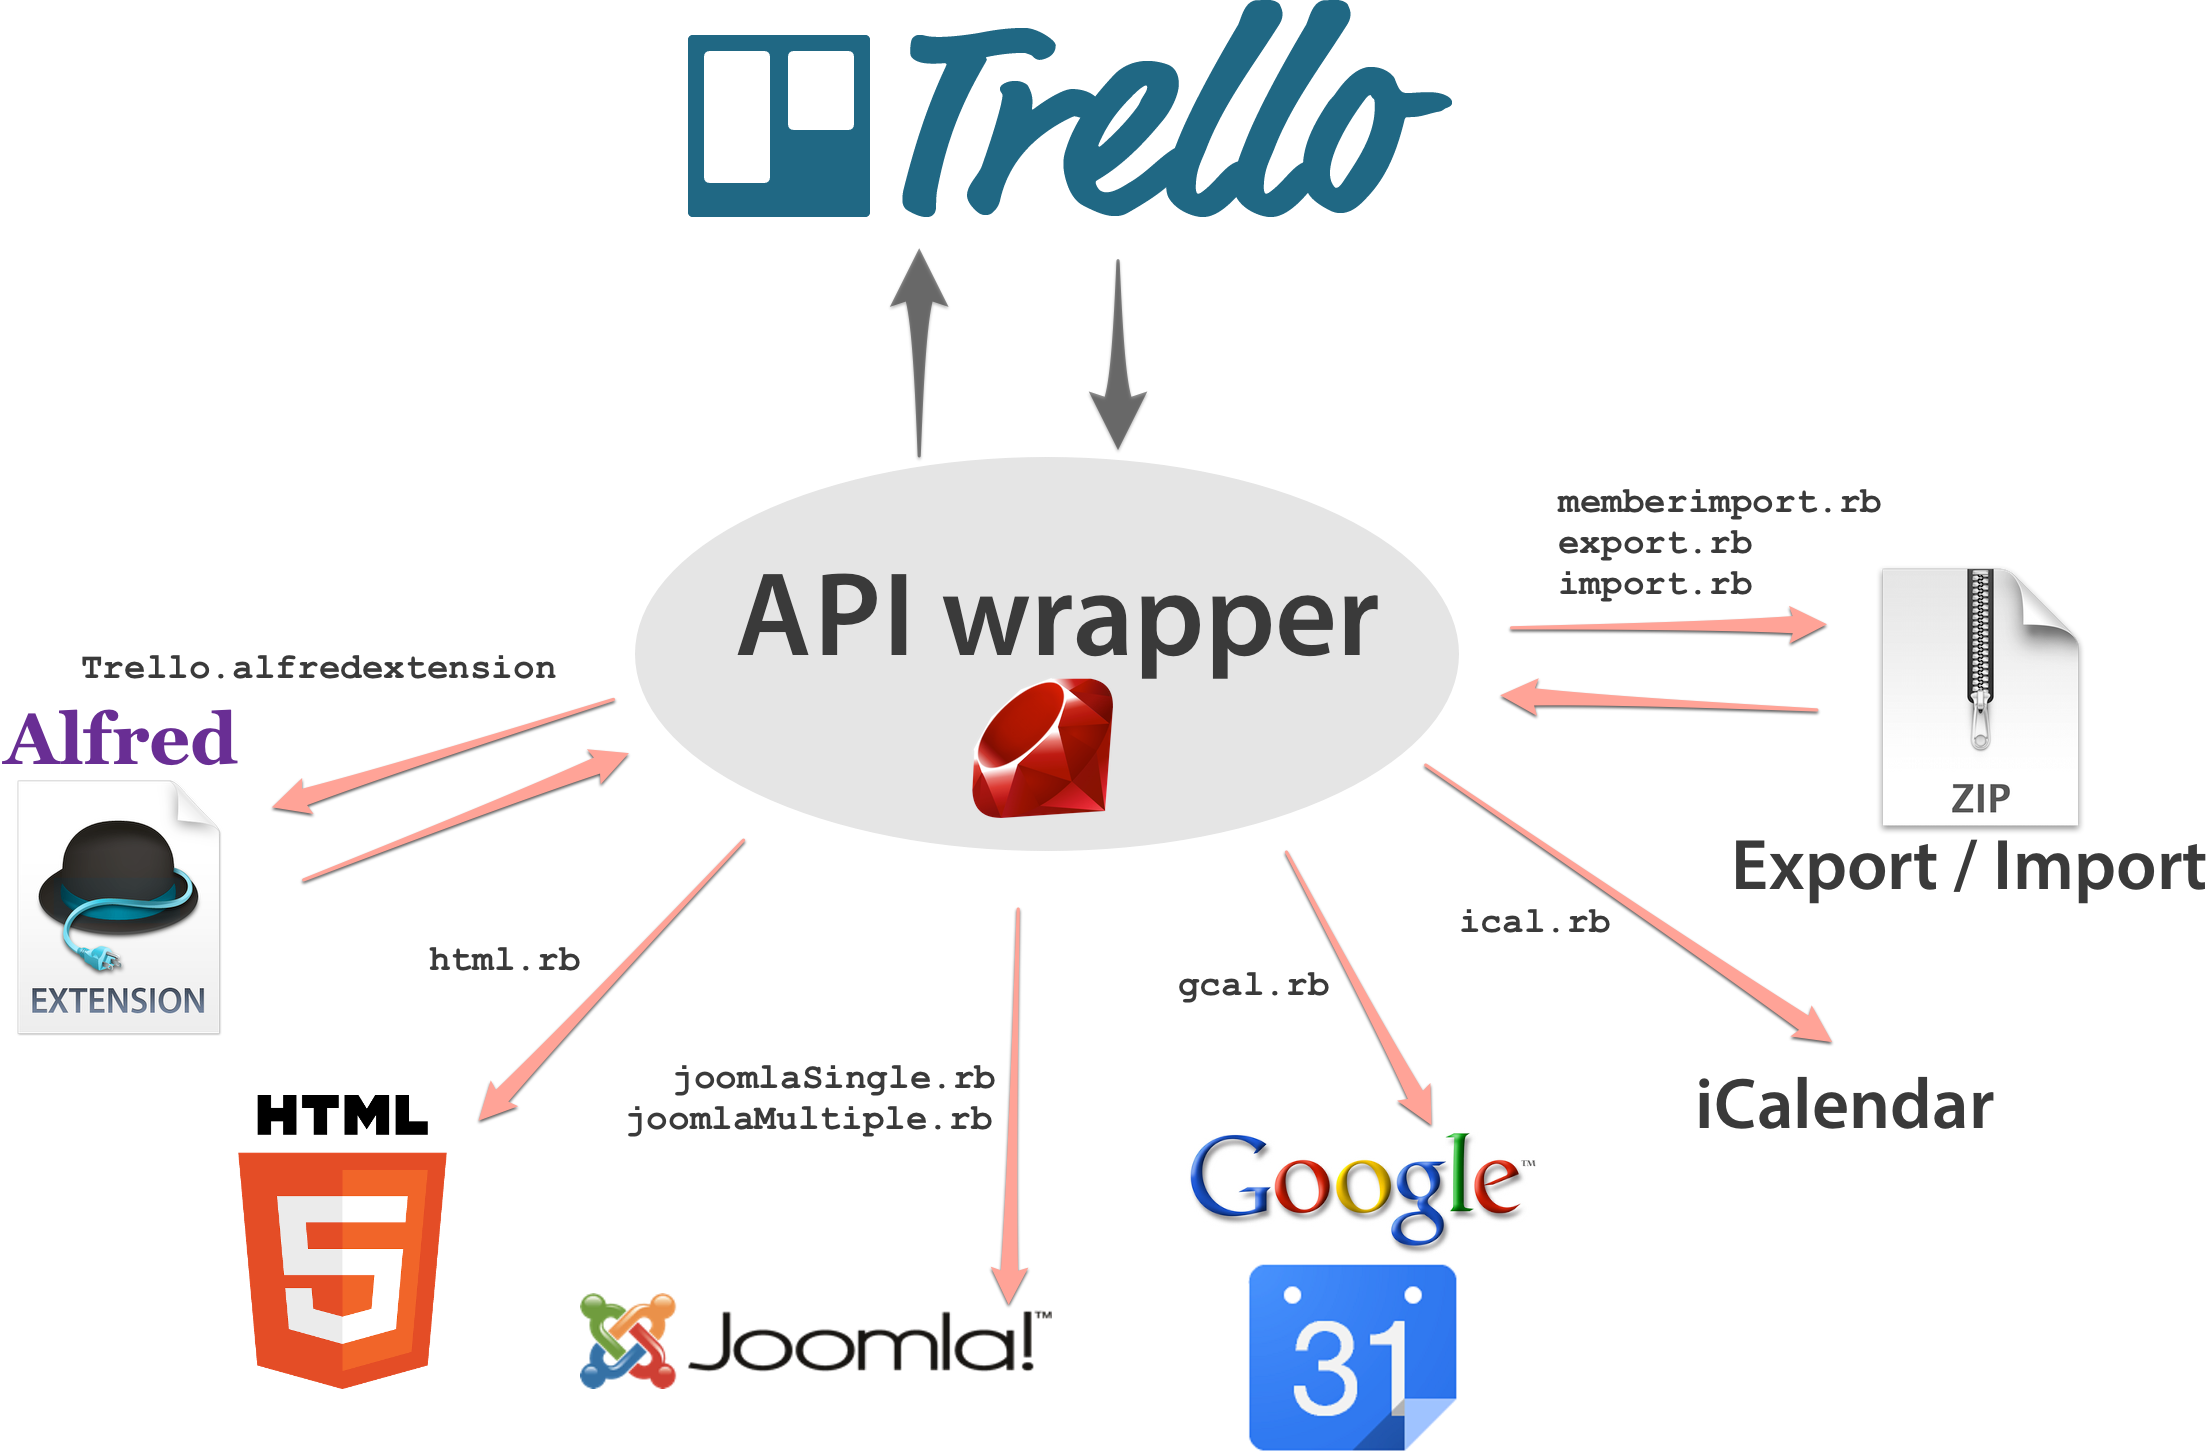
\includegraphics[width=\textwidth]{figures/api-wrapper}
\caption{Connections between Trello, the API wrapper and the actual features. \cite{ruby:icon}\cite{html:logo}\cite{joomla}\cite{google} }
\label{fig: api-wrapper}
\end{figure}

The API wrapper has also functions to pre-process data for Ruby. From a developers point of view, Trello is all about cards. Cards are the only things in Trello with real data, not just meta data. So if the task is so get a board from the API\index{API} it means to get the cards of the board. There is an API call to get all cards which are in a specific board. But with this call the developer doesn't get all information about the cards. So the API wrapper has to execute the API call for a single card to cummulate all information about all cards of the board. This is the function of the API wrapper to keep the actual script clean. So the developer can work with the data and hasn't to worry about determining them.

\section{Handling of date and time}
The cards in Trello may have set due dates. A due date is a date at which the creator of the card thinks it should be done. The due date is represented by the Trello API as an ISO\nomenclature{ISO}{International Organization for Standardization} 8601\index{ISO!8601} formatted string. The timezone\index{timezone} of the date is UTC\nomenclature{UTC}{Universal Time Coordinated}. To ensure that the correct time is displayed always the date has to be adapted to the local time. That's perfeormed with the code in listing \ref{listing021}.

\begin{lstlisting}[aboveskip=1\baselineskip, caption=Response of the token request., label=listing021]
fdate = Time.iso8601(date).getlocal
\end{lstlisting}

It parses the given date string in ISO 8601 format to a Ruby Time object. The \lstinline{getlocal} is the important part here. This function of the Time class determines server's time zone and readjusts the time accordingly. For this function working as intended it's important that the correct time zone is set on the used server. 

\todo{Describe getDate}
